\section {Проектирование и изготовление}

Основные этапы работы:

\begin{itemize}
	\item Проектирование и прототипирование; 
	\item Изготовление деталей;
	\item Сборка;
	\item Разработка управляющей программы
\end{itemize}

\subsection{Проектирование и прототипирование}

\begin{figure}[H]
	\centering
	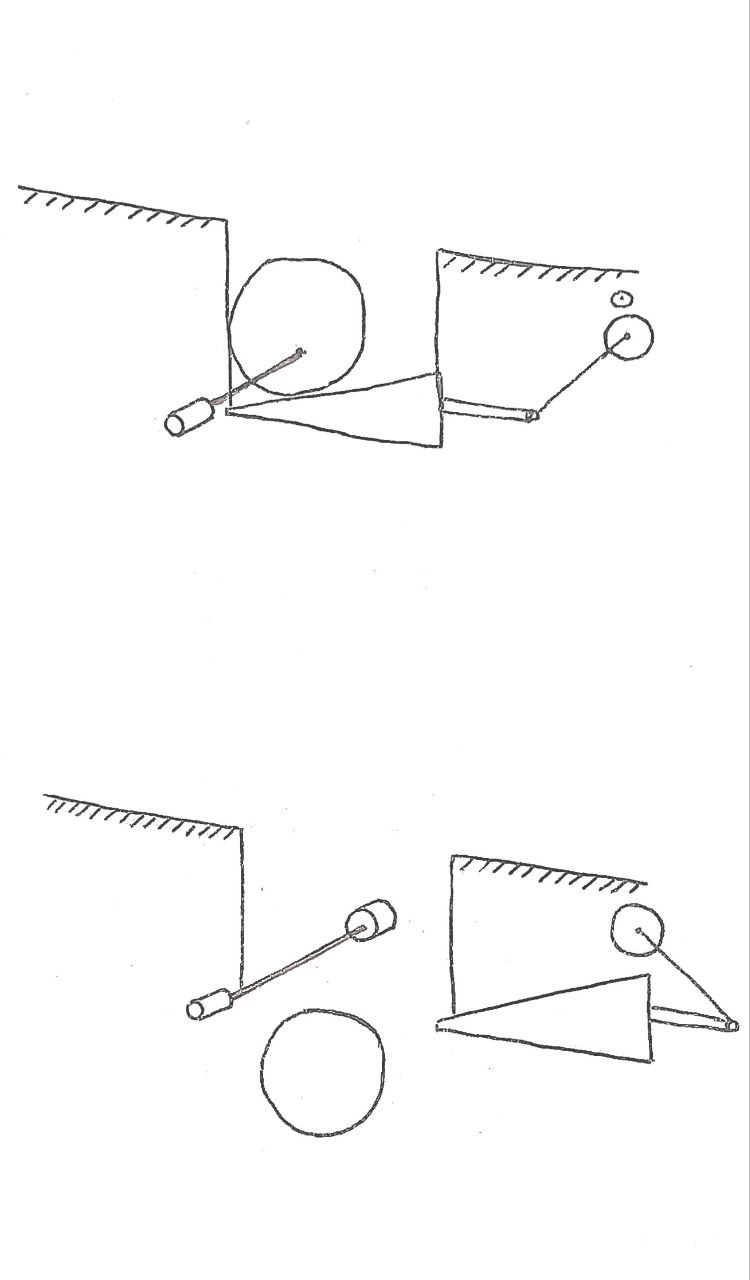
\includegraphics[width=12cm]{scheme_idea.jpg}
	\caption{Принципиальная схема устройства}
	\label{ris:scheme_idea}
\end{figure}
\par\medskip

Принципиальная схема устройства приведена на рис.~\ref{ris:scheme_idea}. Монета падает в щель монетоприемника 1 и перекрывает инфракрасный луч от инфракрасного светодиода 2. Фоторанзистор 5 передает управляющий сигнал на шаговый мотор 3, который приводит в движение клин 4. Когда клин отводится достаточно для того, чтобы монета упала насквозь, инфракрасный луч светодиода 2 перестает перекрываться, что фиксируется фототранзистором. 



По данной принципиальной схеме был собран прототип (см. рис.~\ref{ris:proto}). Он успешно прошел проверку на работоспособность, что позволило нам использовать данный механизм в дальнейшем.

\begin{figure}[H]
	\centering
	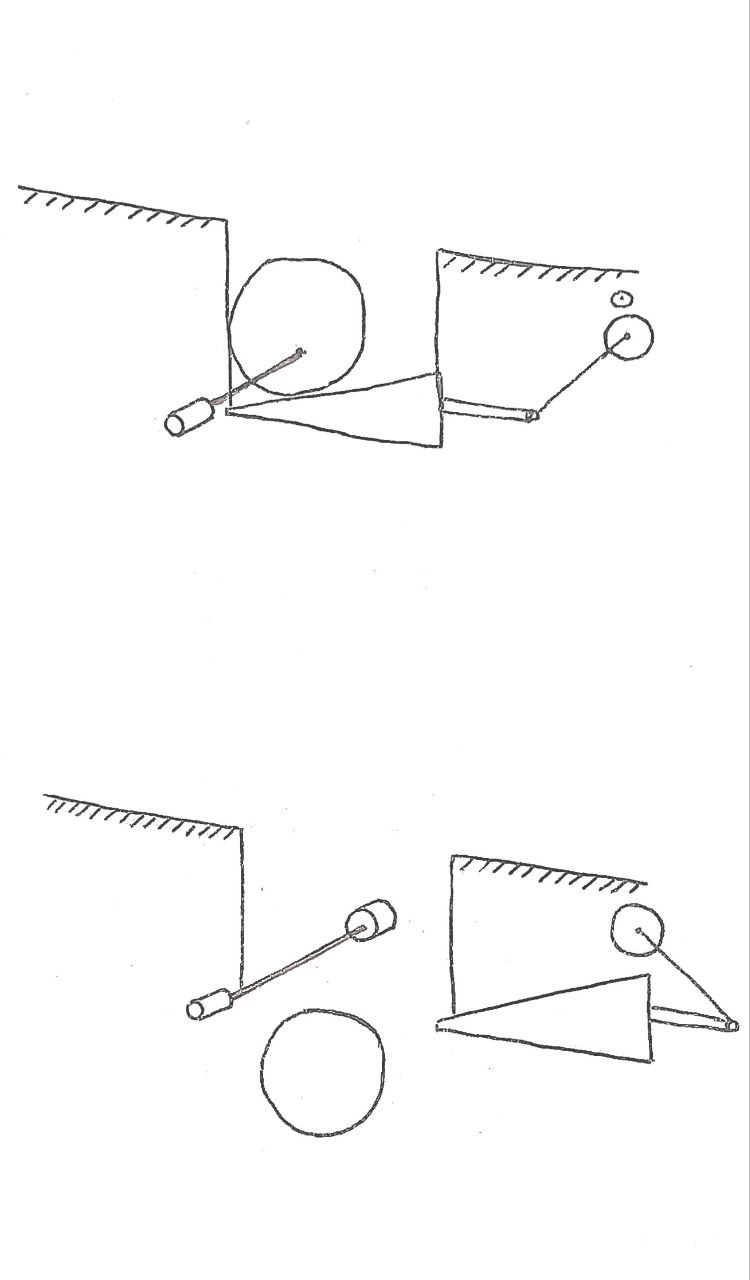
\includegraphics[width=12cm]{scheme_idea.jpg}
	\caption{Прототип}
	\label{ris:proto}
\end{figure}
\par\medskip

При проектировании финальной версии мы доработали механизм затвора для его длины (со 120 мм до 60 мм) (см. рис.~\ref{ris:mechan}).
Корпус копилки состоит из двух основных составных частей - крышки, на которой закреплены все основные детали механизма, и коробки для монет (см. рис.~\ref{ris:korob}). 

\begin{figure}[H]
	\centering
	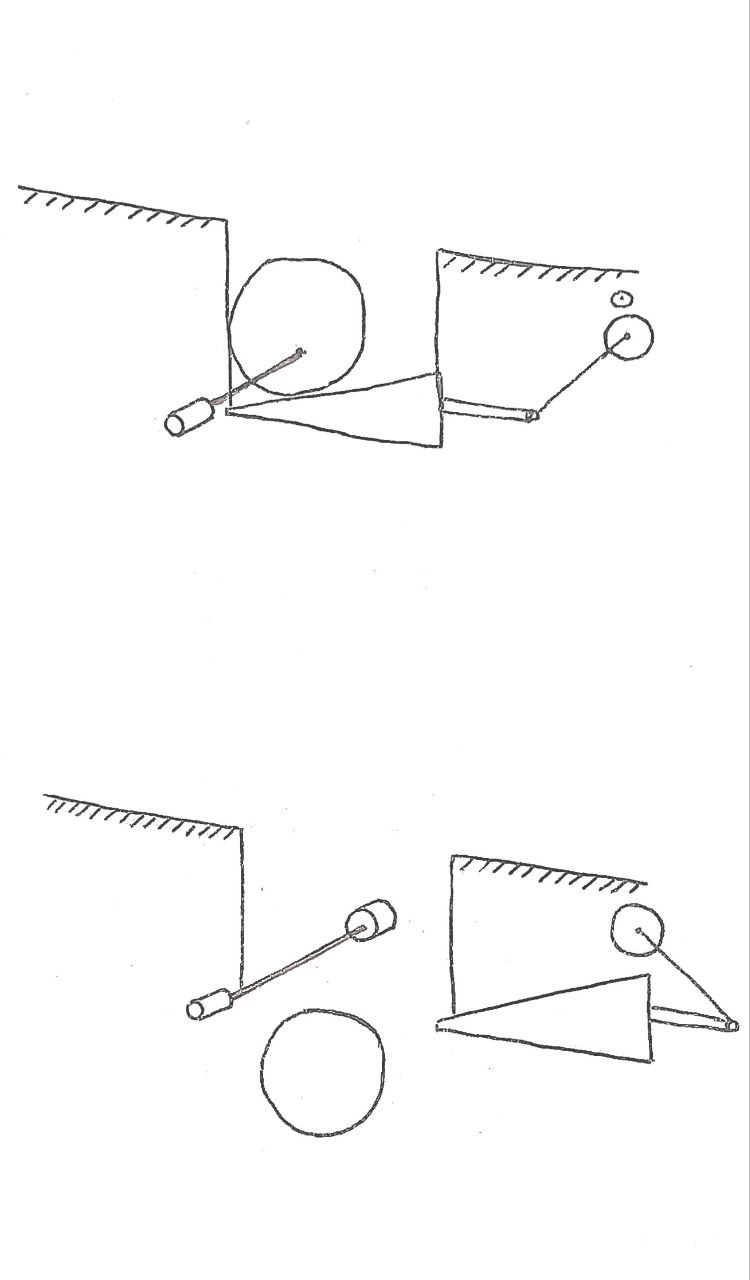
\includegraphics[width=12cm]{scheme_idea.jpg}
	\caption{Реализация механизма}
	\label{ris:mechan}
\end{figure}
\par\medskip

На верхней крышке предусмотрено размещение 2-х кнопок, дисплея, модуля Arduino Nano, драйвера шагового мотора и его драйвера, фототранзистора и инфракрасного светодиода и механизма затвора. Питание осуществляется от постоянного тока 5V от сети (см. рис.~\ref{ris:kryshka_model}, рис.~\ref{kryshka_real}).  

\begin{figure}[H]
	\centering
	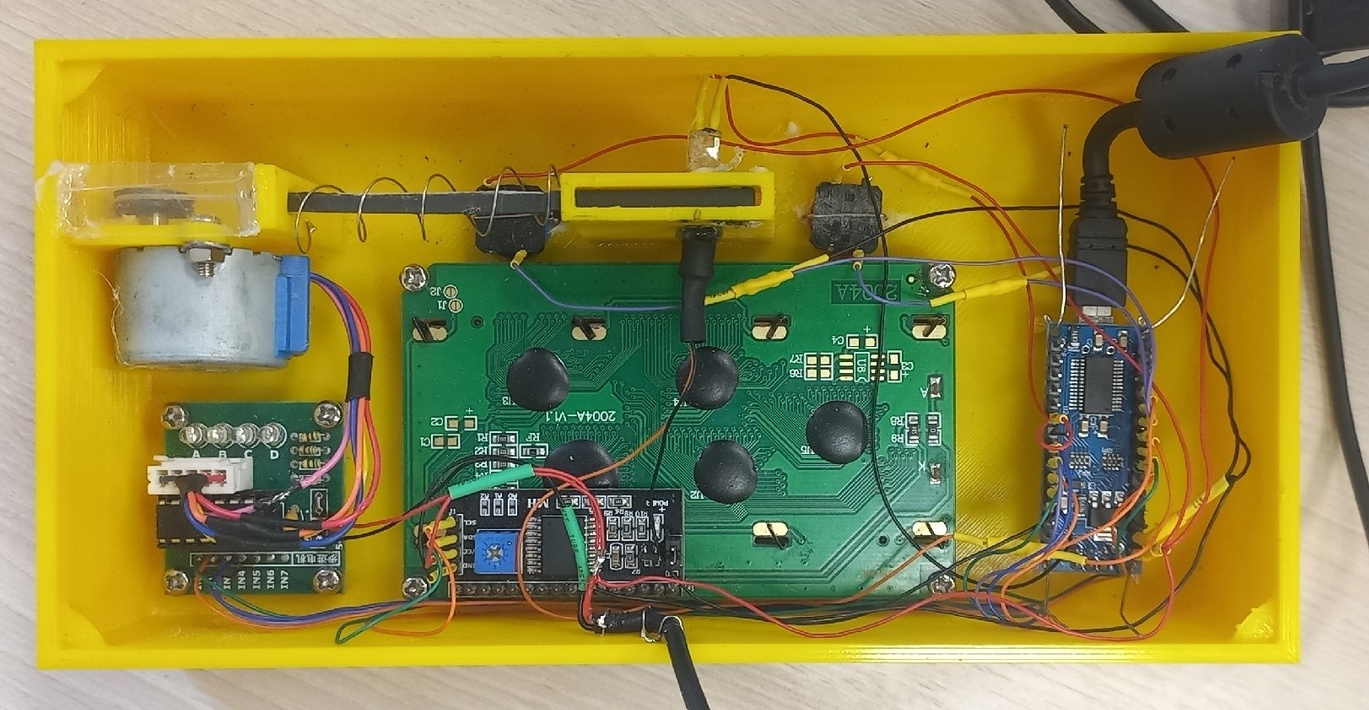
\includegraphics[width=12cm]{kryshka_real.jpg}
	\caption{Крышка -- реализация}
	\label{ris:kryshka_real}
\end{figure}
\par\medskip

\begin{figure}[H]
	\centering
	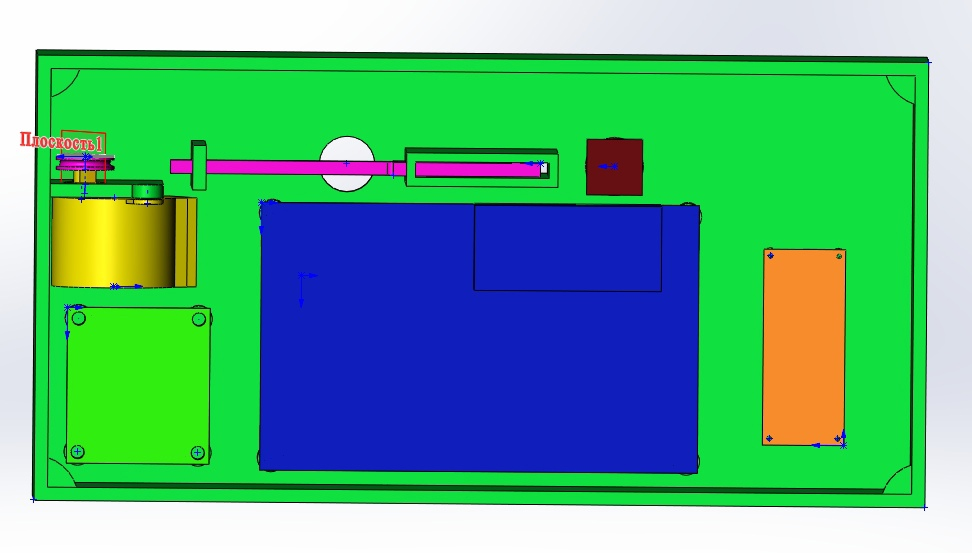
\includegraphics[width=12cm]{kryshka_model.jpg}
	\caption{Крышка -- модель}
	\label{ris:kryshka_model}
\end{figure}
\par\medskip